\documentclass{article}
\usepackage{graphicx}
\usepackage{subcaption}

\begin{document}


\begin{figure}
\centering
  \begin{subfigure}[b]{0.3\textwidth}
    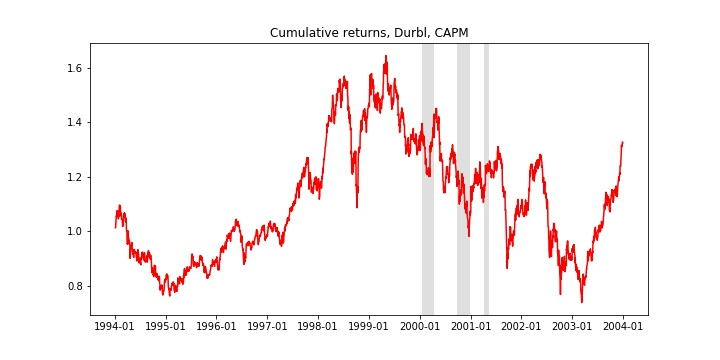
\includegraphics[width=\textwidth]{Durbl/bwunif_full_cumrets_ofint_CAPM.jpg}
    \caption{Durbl, CAPM}
    \label{fig:1}
  \end{subfigure}
  %
  \begin{subfigure}[b]{0.3\textwidth}
    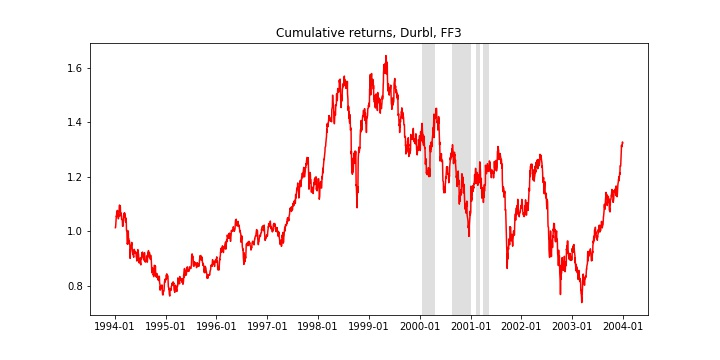
\includegraphics[width=\textwidth]{Durbl/bwunif_full_cumrets_ofint_FF3.jpg}
    \caption{Durbl, FF3}
    \label{fig:2}
  \end{subfigure}
  %
   \begin{subfigure}[b]{0.3\textwidth}
    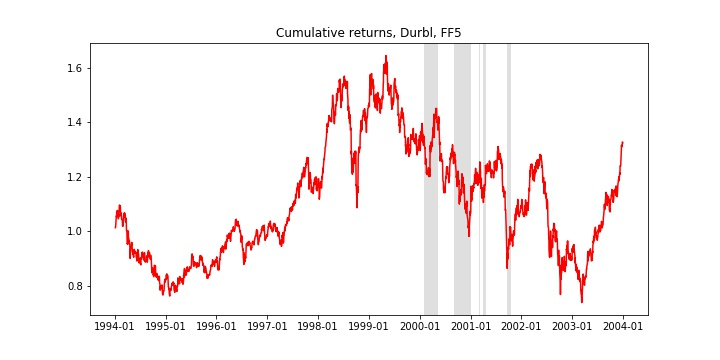
\includegraphics[width=\textwidth]{Durbl/bwunif_full_cumrets_ofint_FF5.jpg}
    \caption{Durbl, FF5}
    \label{fig:2}
  \end{subfigure}
  \end{figure}
 
 \begin{figure}
  \centering
  \begin{subfigure}[b]{0.3\textwidth}
    \centering
    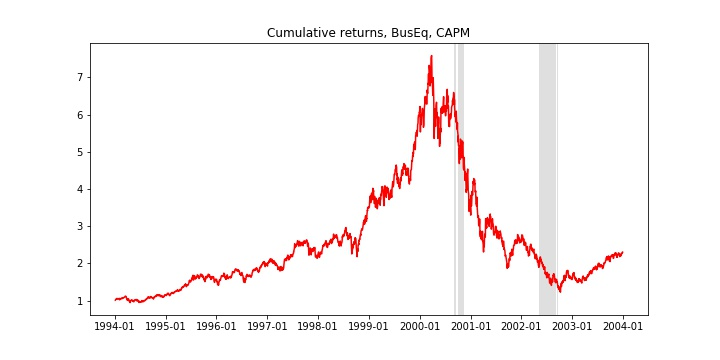
\includegraphics[width=\textwidth]{BusEq/bwunif_full_cumrets_ofint_CAPM.jpg}
    \caption{BusEq, CAPM}
    \label{fig:1}
  \end{subfigure}
  %
  \begin{subfigure}[b]{0.3\textwidth}
    \centering
    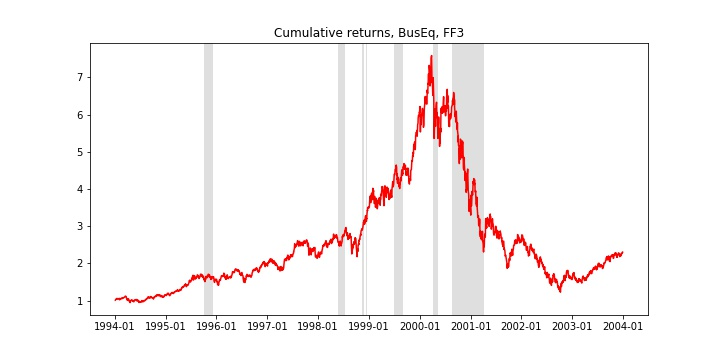
\includegraphics[width=\textwidth]{BusEq/bwunif_full_cumrets_ofint_FF3.jpg}
    \caption{BusEq, FF3}
    \label{fig:2}
  \end{subfigure}
  %
    \begin{subfigure}[b]{0.3\textwidth}
    \centering
    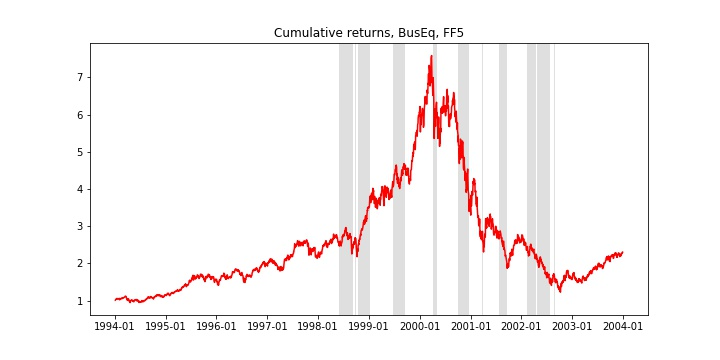
\includegraphics[width=\textwidth]{BusEq/bwunif_full_cumrets_ofint_FF5.jpg}
    \caption{BusEq, FF5}
    \label{fig:1}
  \end{subfigure}
  %
  \end{figure}

 
  \begin{figure}
  \centering
  \begin{subfigure}[b]{0.3\textwidth}
    \centering
    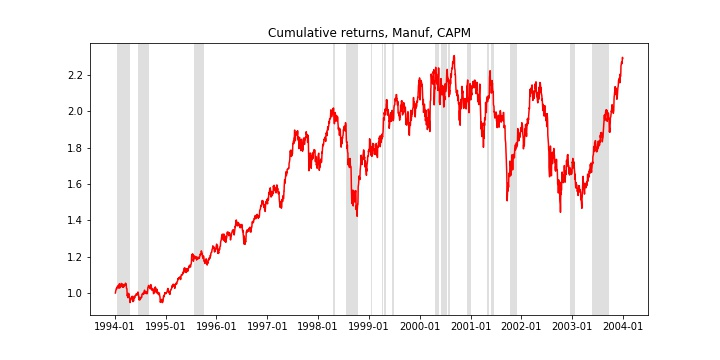
\includegraphics[width=\textwidth]{Manuf/bwunif_full_cumrets_ofint_CAPM.jpg}
    \caption{Manuf, CAPM}
    \label{fig:1}
  \end{subfigure}
  %
  \begin{subfigure}[b]{0.3\textwidth}
    \centering
    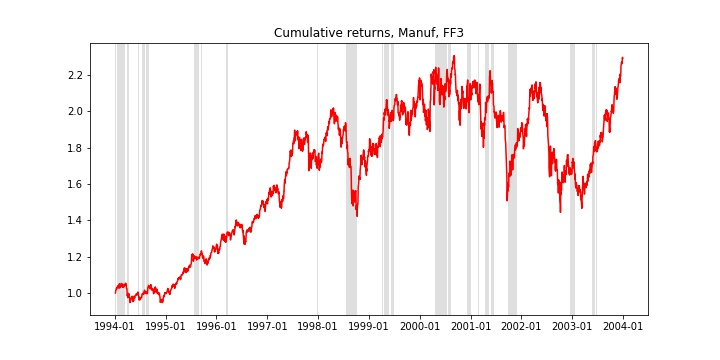
\includegraphics[width=\textwidth]{Manuf/bwunif_full_cumrets_ofint_FF3.jpg}
    \caption{Manuf, FF3}
    \label{fig:2}
  \end{subfigure}
  %
    \begin{subfigure}[b]{0.3\textwidth}
    \centering
    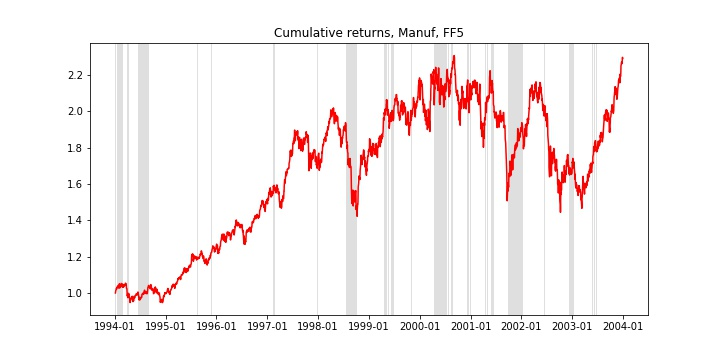
\includegraphics[width=\textwidth]{Manuf/bwunif_full_cumrets_ofint_FF5.jpg}
    \caption{Manuf, FF5}
    \label{fig:1}
  \end{subfigure}
  %
  \end{figure}
  
  \begin{figure}
  \centering
  \begin{subfigure}[b]{0.3\textwidth}
    \centering
    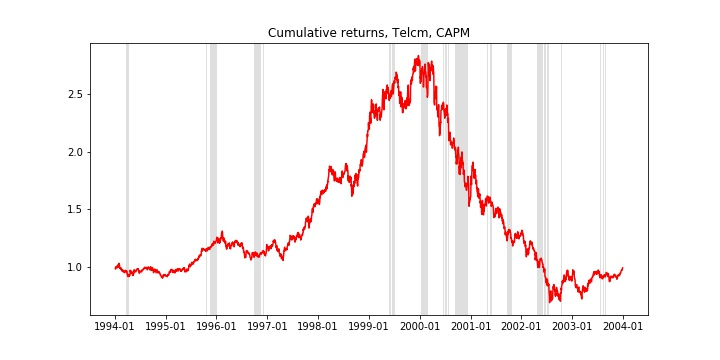
\includegraphics[width=\textwidth]{Telcm/bwunif_full_cumrets_ofint_CAPM.jpg}
    \caption{Telcm, CAPM}
    \label{fig:1}
  \end{subfigure}
  %
  \begin{subfigure}[b]{0.3\textwidth}
    \centering
    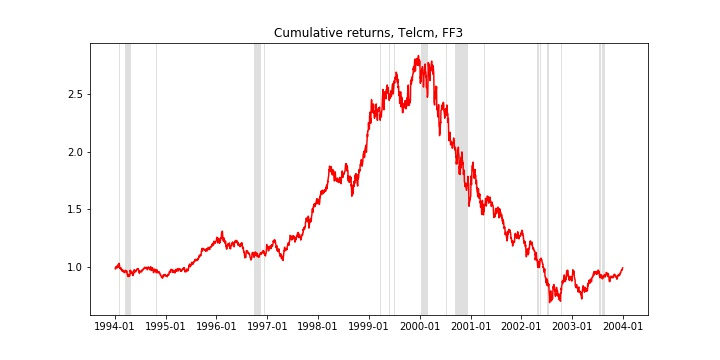
\includegraphics[width=\textwidth]{Telcm/bwunif_full_cumrets_ofint_FF3.jpg}
    \caption{Telcm, FF3}
    \label{fig:2}
  \end{subfigure}
  %
    \begin{subfigure}[b]{0.3\textwidth}
    \centering
    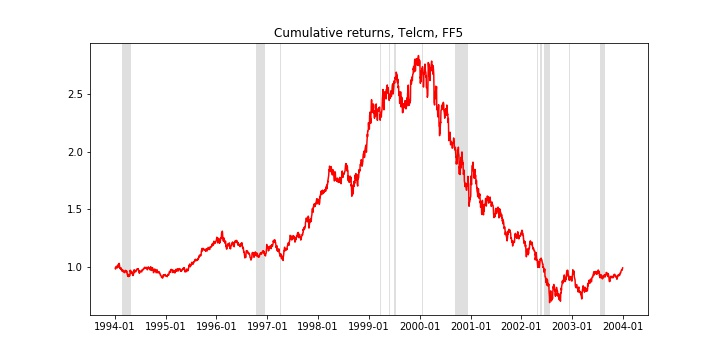
\includegraphics[width=\textwidth]{Telcm/bwunif_full_cumrets_ofint_FF5.jpg}
    \caption{Telcm, FF5}
    \label{fig:1}
  \end{subfigure}
  %
  \end{figure}
  
 \begin{figure}
  \centering
  \begin{subfigure}[b]{0.3\textwidth}
    \centering
    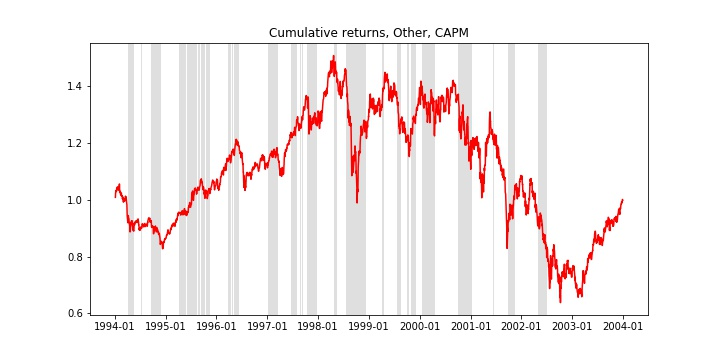
\includegraphics[width=\textwidth]{Other/bwunif_full_cumrets_ofint_CAPM.jpg}
    \caption{Other, CAPM}
    \label{fig:1}
  \end{subfigure}
  %
  \begin{subfigure}[b]{0.3\textwidth}
    \centering
    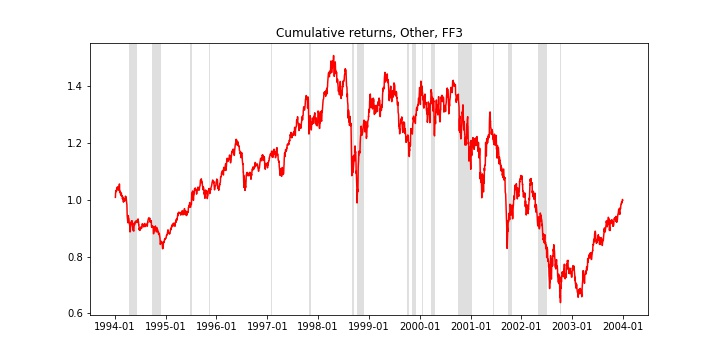
\includegraphics[width=\textwidth]{Other/bwunif_full_cumrets_ofint_FF3.jpg}
    \caption{Other, FF3}
    \label{fig:2}
  \end{subfigure}
  %
    \begin{subfigure}[b]{0.3\textwidth}
    \centering
    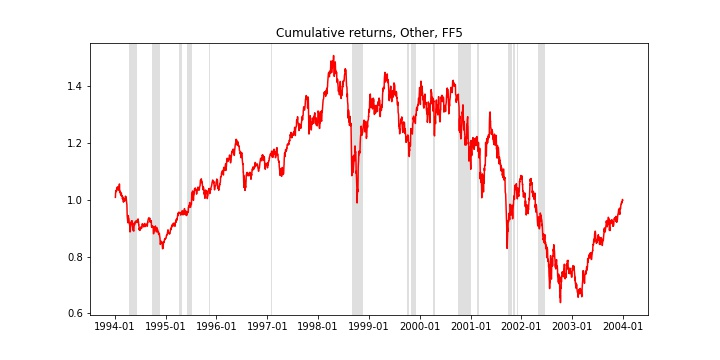
\includegraphics[width=\textwidth]{Other/bwunif_full_cumrets_ofint_FF5.jpg}
    \caption{Other, FF5}
    \label{fig:1}
  \end{subfigure}
  %
  \end{figure}
        
  \end{document}
  
  